\documentclass[]{scrreprt}

\usepackage{lipsum} % only for the example

% header on scrreprt
\usepackage[automark,headsepline]{scrlayer-scrpage}
\clearpairofpagestyles
\rofoot{\pagemark}
\lehead{\headmark}
\rohead{\headmark}
\pagestyle{scrheadings}

% paper size
\usepackage[
	hscale=0.74,
	vscale=0.85,
	heightrounded,
	includehead
]{geometry}

\usepackage{subfig}
\usepackage{float}

\usepackage{scrhack}
\usepackage{listings}
\usepackage{graphicx}
\usepackage[bookmarks=true]{hyperref}
\usepackage[utf8]{inputenc}
\hypersetup{
    bookmarks=false,    % show bookmarks bar?
    pdftitle={Software Requirement Specification},    % title
    pdfauthor={Jean-Philippe Eisenbarth},                     % author
    pdfsubject={TeX and LaTeX},                        % subject of the document
    pdfkeywords={TeX, LaTeX, graphics, images}, % list of keywords
    citecolor=black,       % color of links to bibliography
    filecolor=black,        % color of file links
	colorlinks,
	urlcolor=[rgb]{0,0.5,0.5},
    linkcolor=[rgb]{0,0.5,0.5},
    linktoc=page            % only page is linked
}%
\def\myversion{1.1 }
%\title

% first line indent
\usepackage{indentfirst}
\usepackage{import}

% nice quotation
\usepackage{csquotes}

% color support
\usepackage[dvipsnames]{xcolor}
% \ast symbol
\usepackage{latexsym}

\usepackage{multirow}

\usepackage{array}
\newcolumntype{L}[1]{>{\raggedright\let\newline\\\arraybackslash\hspace{0pt}}p{#1}}
\newcolumntype{C}[1]{>{\centering\let\newline\\\arraybackslash\hspace{0pt}}p{#1}}
\newcolumntype{R}[1]{>{\raggedleft\let\newline\\\arraybackslash\hspace{0pt}}p{#1}}

\begin{document}

\begin{flushright}
	\rule{14cm}{2pt}
	\vskip1cm
	\begin{bfseries}
		\Huge{Software Requirements Specification\\Documentation}\\
		\vspace{1.5cm}
		for\\
		\vspace{1.5cm}
		ICDE-ScholarHub\\
		\LARGE{Version \myversion}\\
		\vspace{1.5cm}
		Prepared by : \\
		Zerui Wang\\
		{\small 40177315}\\
		Ding Li\\
		{\small 40160073}\\
		Jun Huang\\
		{\small 40168167}\\
		\vspace{1.5cm}
		{\footnotesize last editing: \today}
	\end{bfseries}
\end{flushright}

\thispagestyle{empty}

\tableofcontents

\thispagestyle{empty}

\chapter{Introduction}

\section{Purpose}

\noindent
We define a system named \textbf{ICDE-ScholarHub} which is a web-based Paper Search Engine with ICDE concepts implemented.

The system will practice the idea of ICDE to help the researchers work more efficiently regarding user operation history, teamwork, and paper trending.

Furthermore, the system exposes the API of ICDE for the development of 3rd-party applications or plugins.


\section{Sytem Problem Statement}

\noindent
During the daily research work, it always happens that researchers forget some critical paper they have read on the web-based paper search system a long-time ago. It takes time to find the critical one from the huge amount of paper list from a different academic area.

More sadly, people may miss the latest paper which is important to their research. Researchers have supervisors, colleagues, and teammates. They like to share the latest paper in the same area with the team. But they do not want to disturb others by sending papers through email too often and it is not well organized.

If there is a  system that implements ICDE API, the reading history will be well recorded. The system will log down every activity the user performed.

For example, the researcher can develop a small tool to log down his paper reading history; the research team can develop a tool for sharing team member’s paper reading history,  paper marking history, area preference, and so on.

The aim of using ICDE-ScholarHub on the paper search system is to help the researchers and their teams work in a more efficient way.

\section{References}

\noindent
\textbf{ICDE: } \url{https://www.researchgate.net/publication/220690558_Essential_Software_Architecture_2_ed}
% {Essential\_Software\_Architecture\_2\_ed}

\chapter{Overall Description}

\import{./section/user-scenario-user-story}{usus.tex}

\import{./section/system-requirements-specification}{srs.tex}

\import{./section/system-architecture-design}{sad.tex}

\import{./section/system-modeling}{sm.tex}

\import{./section/operating-environment}{oe.tex}

\chapter{Functional Requirements Specification}

\import{./section/functional-requirements-specification}{frs0.tex}

\import{./section/functional-requirements-specification}{frs1.tex}

\def\apda{Appendix A: Glossary}
\chapter*{\apda}
\addcontentsline{toc}{chapter}{\apda}

{\parindent0pt

	\textbf{ICDE:} stands for Information Capture and Dissemination Environment.

	\textbf{Researcher:} academic researcher with needs a paper search engine to help their research work.

	\textbf{Researche Team:} a team of researcher.

	\textbf{Paper:} academic papers which stored in the system.

	\textbf{SRS:} stands for system requirements specification.

	\textbf{FRS:} stands for functional requirements specification.

	\textbf{MVC:} stands for Model-View-Controller design pattern.

	\textbf{BO:} stands for business object for class diagram design.

}

\def\apdb{Appendix B: Editing Records}
\chapter*{\apdb}
\addcontentsline{toc}{chapter}{\apdb}

\begin{itemize}
	\item \textbf{v1.0} Jun Huang - 02/11/2021
	\item \textbf{v1.5} Jun Huang - 03/11/2021
\end{itemize}

\def\apdc{Appendix C: Prototype of WebUI}
\chapter*{\apdc}
\addcontentsline{toc}{chapter}{\apdc}

\begin{figure}[htbp]
	\centering
	\begin{minipage}[t]{0.48\textwidth}
		\centering
		
\includegraphics[width=6cm]{./section/appendix/img/UI Home page.jpg}
		\caption{Home Page UI}
	\end{minipage}
	\begin{minipage}[t]{0.48\textwidth}
		\centering
		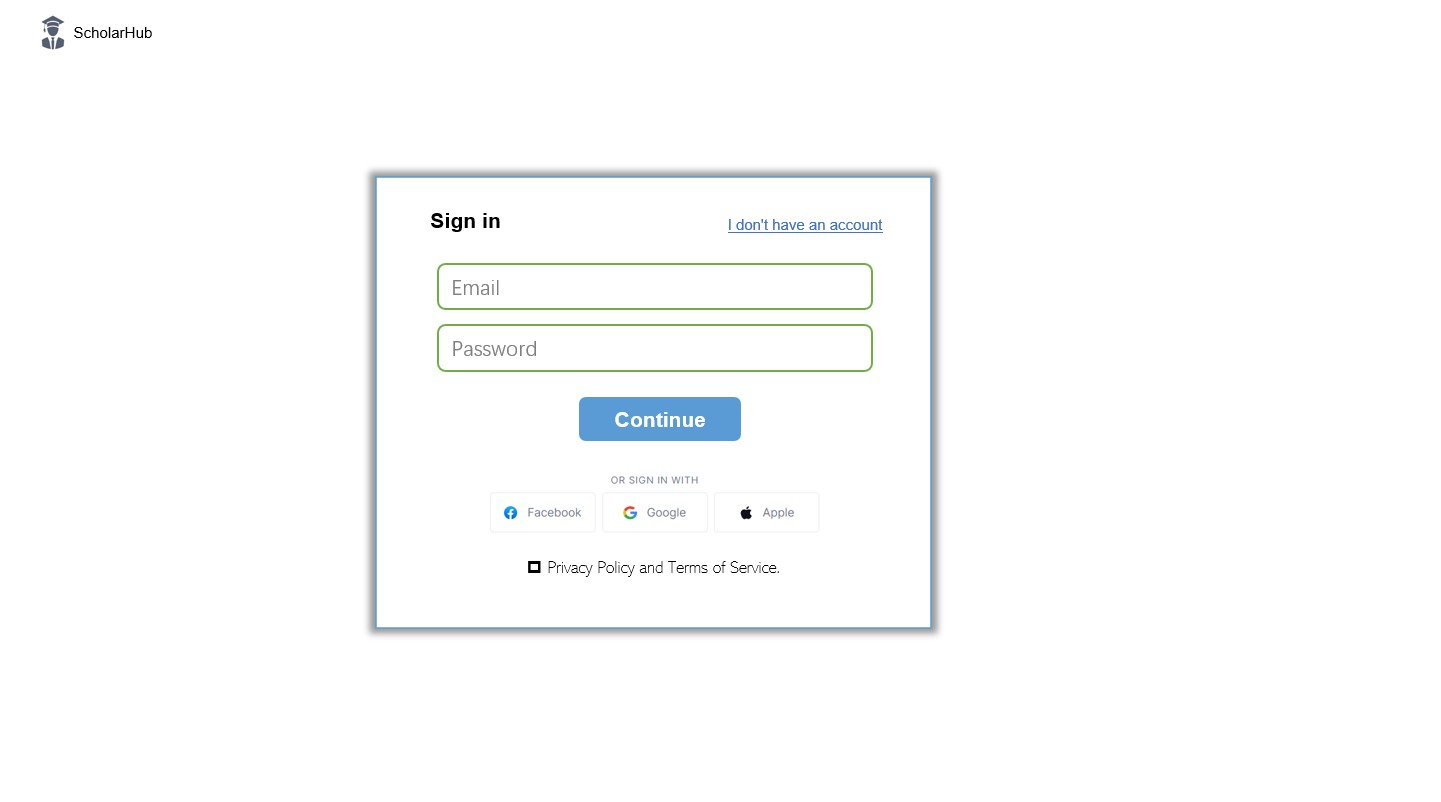
\includegraphics[width=6cm]{./section/appendix/img/UI sign in.jpg}
		\caption{Sign in UI}
	\end{minipage}
\end{figure}

\begin{figure*}[htp]
	\centering
	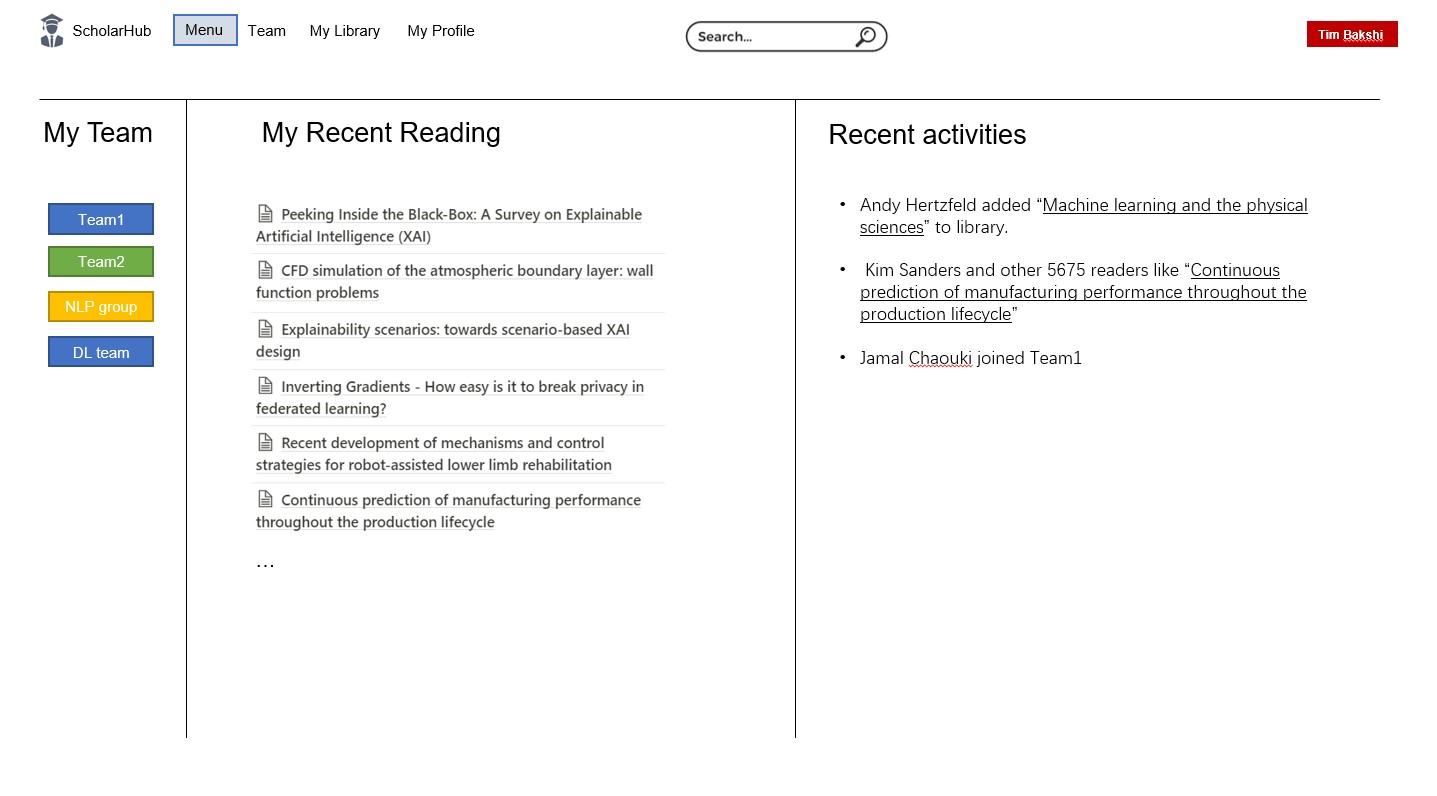
\includegraphics[width=\textwidth]{./section/appendix/img/UI MainPage.jpg}
	\caption{Menu Page UI}
	\label{fig:Memu Page}
\end{figure*}

\begin{figure*}[htp]
	\centering
	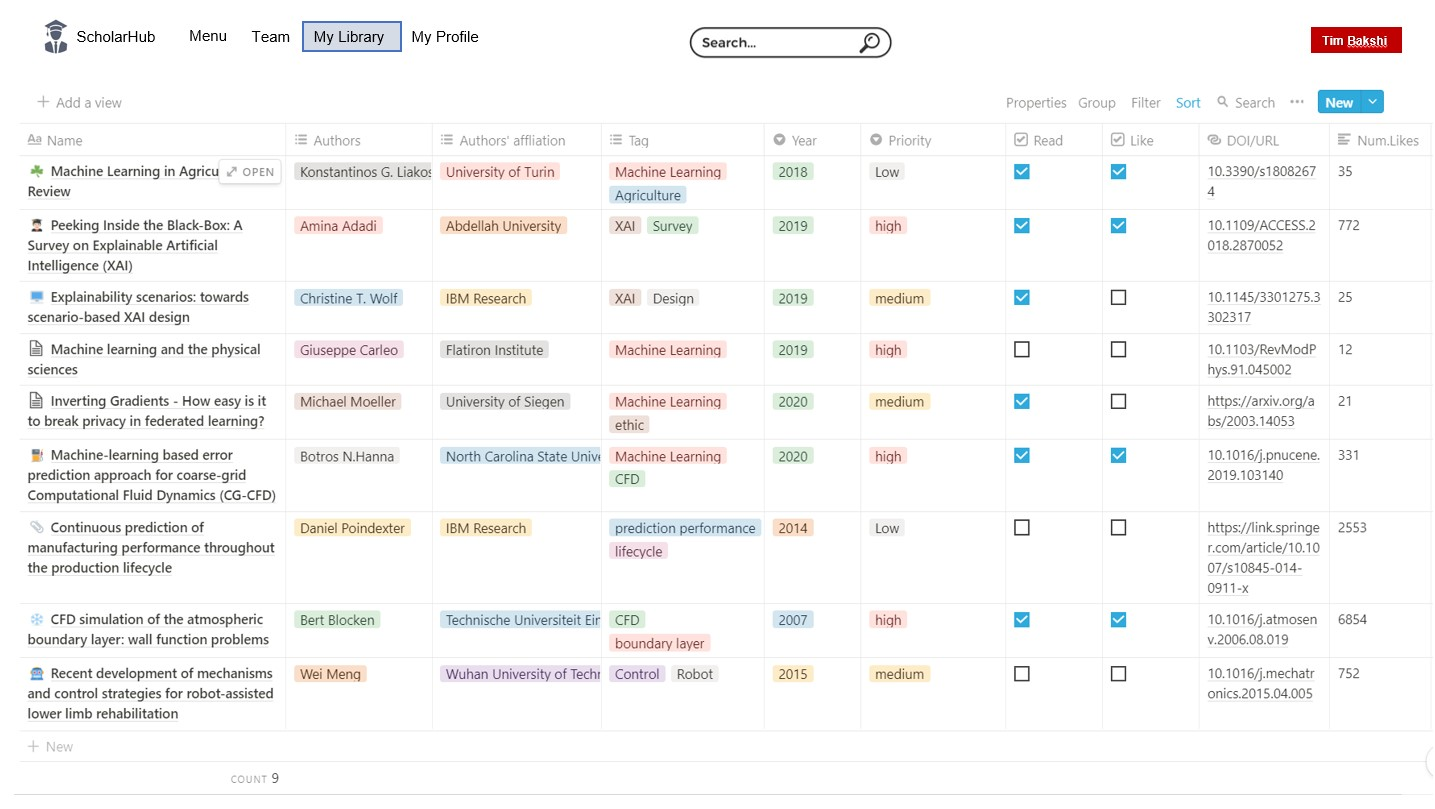
\includegraphics[width=\textwidth]{./section/appendix/img/UI My Library.jpg}
	\caption{My Library UI}
	\label{My Library UI}
\end{figure*}


\begin{figure*}[htp]
	\centering
	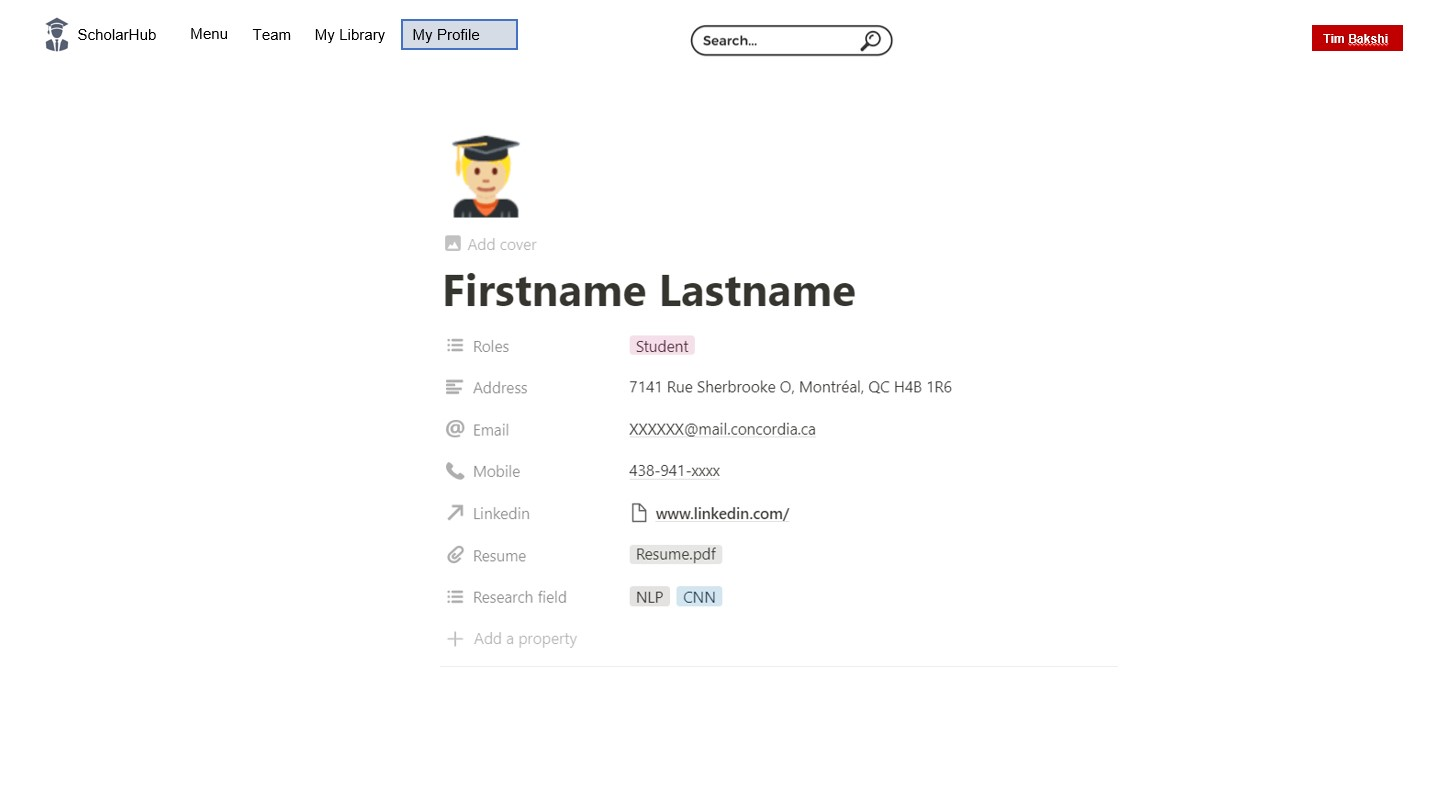
\includegraphics[width=\textwidth]{./section/appendix/img/UI my profile.jpg}
	\caption{My Profile UI}
	\label{my profile UI}
\end{figure*}

\begin{figure*}[htp]
	\centering
	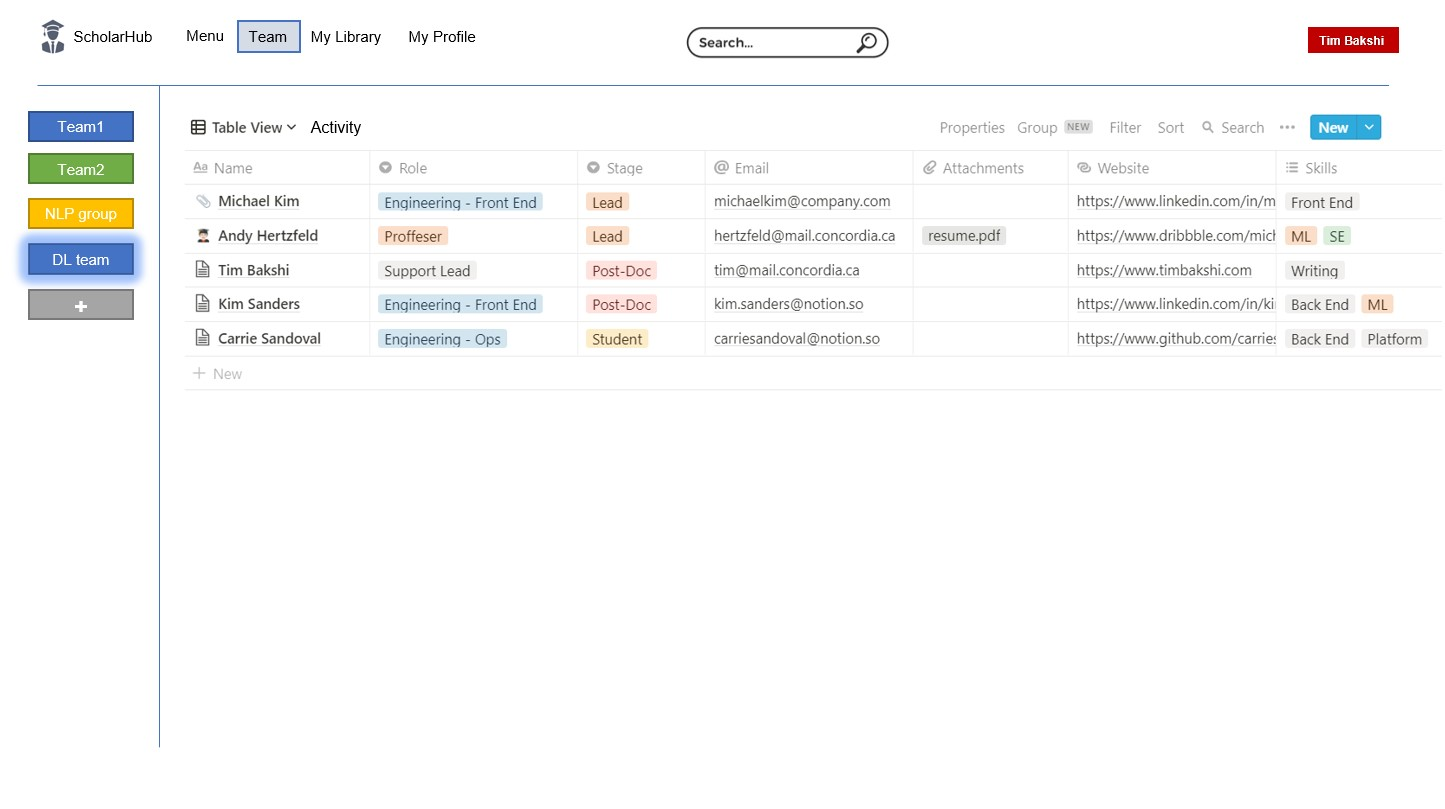
\includegraphics[width=\textwidth]{./section/appendix/img/UI teamlist.jpg}
	\caption{Team List UI}
	\label{teamlist UI}
\end{figure*}

\begin{figure*}[htp]
	\centering
	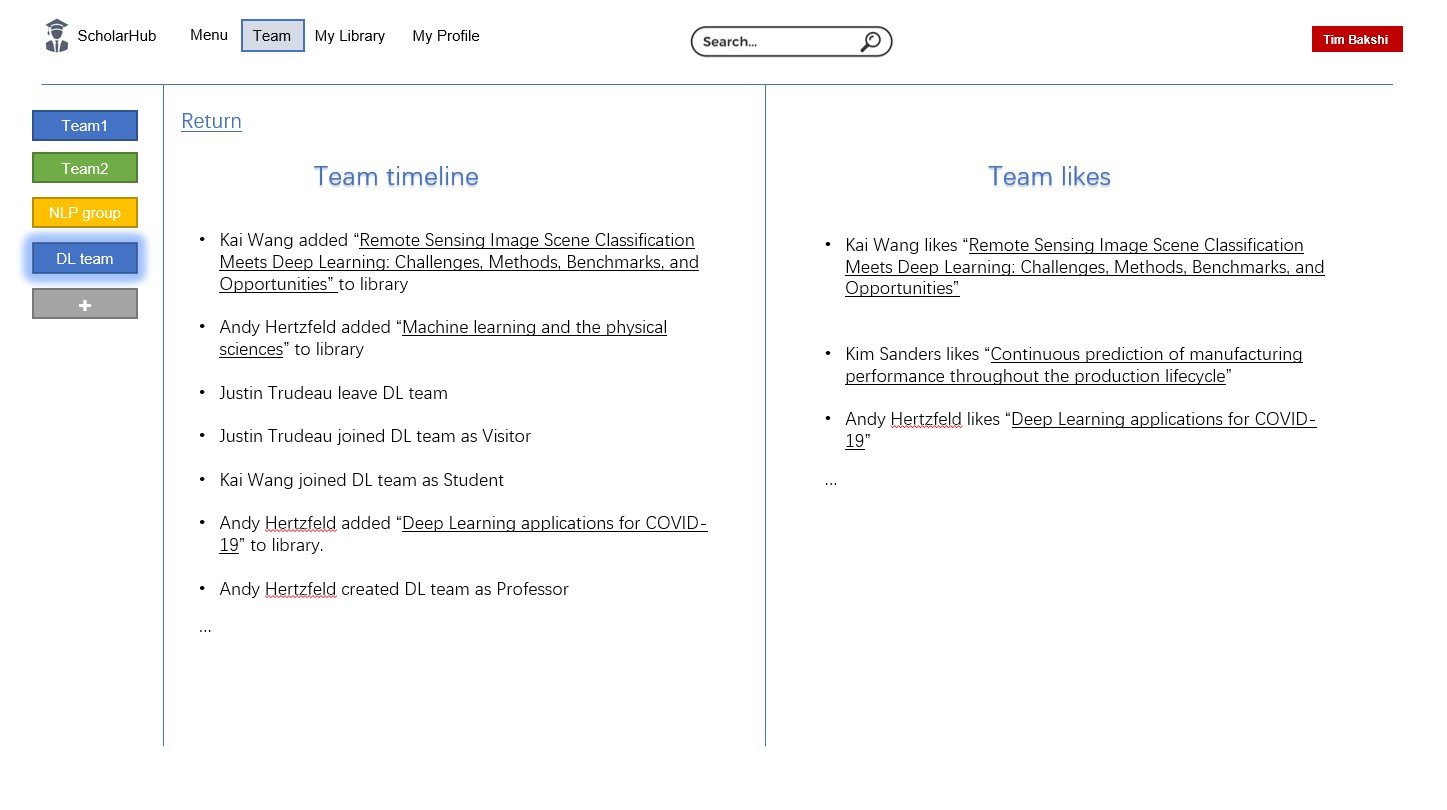
\includegraphics[width=\textwidth]{./section/appendix/img/UITeamactivity.jpg}
	\caption{Team Activity UI}
	\label{Teamactivity UI}
\end{figure*}

% \section{Security Requirements}

\end{document}